\documentclass[10pt,twocolumn,letterpaper]{article}

\usepackage{cvpr}
\usepackage{times}
\usepackage{epsfig}
\usepackage{graphicx}
\usepackage{amsmath}
\usepackage{amssymb}
\usepackage{wrapfig}

% Include other packages here, before hyperref.

% If you comment hyperref and then uncomment it, you should delete
% egpaper.aux before re-running latex.  (Or just hit 'q' on the first latex
% run, let it finish, and you should be clear).
\usepackage[pagebackref=true,breaklinks=true,letterpaper=true,colorlinks,bookmarks=false]{hyperref}

\cvprfinalcopy % *** Uncomment this line for the final submission

\def\cvprPaperID{1} %
\def\httilde{\mbox{\tt\raisebox{-.5ex}{\symbol{126}}}}

% Pages are numbered in submission mode, and unnumbered in camera-ready
\ifcvprfinal\pagestyle{empty}\fi

\begin{document}

%%%%%%%%% TITLE
\title{Practical AutoAugment: Measuring the Impact of AutoAugment on Classification Performance for Additional Image Datasets}

\author{Quoc N. Le, Rounak Mehta, Vikram Natarajan, Anna Novakovska\\
Columbia University\\
{\tt\small \{qnl2000,rm3652,vsn2113,an2915\}@columbia.edu}
\\
}

\maketitle
%\thispagestyle{empty}

%%%%%%%%% ABSTRACT
\begin{abstract}
The AutoAugment [1] authors show how automatically-selected policies for data augmentation can improve on benchmark classifier performance on CIFAR-10, CIFAR-100, SVHN, and ImageNet datasets.  In this paper, we put ourselves in the shoes of practioners seeking to use AutoAugment to improve image classification performance on their own real-world datasets.

The first practical approach to unlocking the value of AutoAugment, as shown by the original paper authors [1], is to "transfer" augmentation policies found for CIFAR-10, SVHN, etc to our own image datasets.  We report mixed results for using transfer learning approach on two additional image datasets: the “Iceberg” dataset from the Kaggle “Statoil/C-CORE Iceberg Classifier Challenge" and the "QuickDraw" dataset from the Kaggle "Quick, Draw! Doodle Recognition Challenge".  For the Iceberg dataset we achieved immediate gains by (1) transfering CIFAR-10 policies which resulted in a 2.6 percent improvement in log loss of our baseline, (2) transfering SVHN policies directly which resulted in a 5.1 percent improvement over our baseline, and (3) transfering manually selected SVHN policies which resulted in a 15.1 percent improvement over our baseline.  For the QuickDraw dataset, however, we did not measure any gains, in fact we struggled to improve our baseline using augmentation.  Our conclusion is that gains from transfer learning using AutoAugment depends on the dataset, although the gains can be impressive and very straightforward as they were with the Iceberg dataset.  Therefore, practioners should certainly consider AutoAugment transfer in their model optimization.

The second approach to unlocking value in AutoAugment is to leverage the AutoAugment [1] reinforcement learning framework to discover optimal policies on additional datasets.  We found, however, that it is difficult to reproduce the reinforcement learning implementation described in the paper, due to no code reference for that implementation and due to lack of GPU resources.  We instead developed an approach we call Simplified AutoAugment, where we implemented a “Random Search Controller” which is a simplification on the Reinforcement Learning Controller, or mechanism for suggesting good policies, in the original paper [1].  We find that our Random Search Controller is able to achieve 3.40 percent error on the CIFAR-10 Wide-Res-Net benchmark, which is an improvement on the no-augmentation baseline of 3.87 percent.  However, the Random Search Controller does not do as well as the Reinforcement Learning Controller from [1], which has a 2.68 percent error rate.  Still, we conclude that an Random Search approach can provide a practical alternative for practioners for automatically finding augmentation policies that improve on a classifier baseline.

\end{abstract}

%%%%%%%%% BODY TEXT
\section{Introduction}

AutoAugment shows the potential for automatically discovering data augmentation techniques that can be “learned” from the image dataset itself. It is a reinforcement learning algorithm which finds optimal policies for data augmentation for training deep learning algorithms. It works by setting the problem up as a discrete search problem, where each policy in the search space corresponds to five sub-policies (each having 2 operations). Reinforcement Learning is used to find optimal policies, then these policies are used to augment a dataset before training with a selected neural network architecture.

The original AutoAugment paper [1] demonstrated the performance of AutoAugment on benchmark datasets such as CIFAR-10, CIFAR-100, SVHN, and ImageNet, and they also showed that learned policies do transfer to other datasets.   That is, the optimal augmentation policies learned to optimize classifier performance on one image dataset will “transfer” or improve classifier performance on a different dataset.   We will measure this transferability onto additional datasets, in particular the Iceberg and Human Protein datasets described in a subsequent section.  The results for this is summarized in the “Preliminary Results - Transfer Learning” section.

However, to learn these policies, the authors use a Reinforcement Learning algorithm whose implementation is not made available with their paper [1].  Therefore we experiment with a "Simplified AutoAugment" approach, where we search over the space of possible policies using a Random Search.  This is a simplified approach because we avoid the complexities of implementing the Reinforcement Learning, although the trade off is likely a smaller positive impact on classifier performance.  Nonetheless, the Random Search is suggested by the AutoAugment [1] authors as a possible research direction that could yield competitive results to Reinforcement Learning. The results for this is summarized in the “Preliminary Results - Learning Policies” section.

\section{Previous Work}

The original AutoAugment paper [1] has a github project that shows the application of the discovered augmentation policies to training the classifiers for CIFAR-10 and CIFAR-100.  There are also a number of github repositories that attempt to reproduce the results of the original paper (DeepVoltaire/AutoAugment, rpmcruz/autoaugment, dnddnjs/pytorch-cifar10).  However, none of these repositories successfully provides an implementation that reproduces the results of the Reinforcement Learning algorithm of the original paper.

The rpmcruz/AutoAugment github repository [3], however, provides the most useful attempted implementation of the Reinforcement Learning approach in the original paper.  This repo leverages the Reinforcement Learning implementations details from two papers [1-2], and in doing so it at least provides a Controller and Child framework for policy searches, where the Controller suggests policies while the Child tests the effect of the policy on training the network.  This was useful to us as we can plug in experimental Controllers that perform a Random Search of policies, for example.

\section{Datasets}

We chose image datasets from Kaggle based on the following criteria:

\begin{itemize}
  \item Image dataset is labeled, i.e. classification is the goal
  \item Image dataset is of a manageable size (less than 10GB)
  \item A Kaggle Kernel is available (ensures repeatability)
  \item Kernel is a single model that can be run relatively quickly (under 1 hour).  (Note this excludes many competition-winning models which are large ensembles and take days to run).
\end{itemize}

The datasets that met these criteria include:

\begin{itemize}
  \item \textbf{Iceberg Dataset}.  This is an image dataset from the Kaggle “Statoil/C-CORE Iceberg Classifier” Challenge.  It contains 1,674 "images" of icebergs and ships that come from radar readings.  
  \item \textbf{QuickDraw Dataset}.  TODO: Add Description
  \item \textbf{CIFAR-10 Dataset}.  This is the same dataset used by the authors [1].  We use this for comparing the Simplified AutoAugment performance to that of the Reinforcement Learning AutoAugment.  Although this dataset is not a Kaggle dataset, it is labeled, relatively small, and has many classifier baselines as specified in the AutoAugment paper [1].        
\end{itemize}


\section{Evaluation Criteria}

\subsection{Transfer Learning}

To measure \textbf{Transfer Learning} on augmentation policies, we will evaluate the following on the Iceberg and Human Protein datasets:

\begin{itemize}
  \item Performance of the classifier baseline (Kaggle Kernel) without any data augmentation.  This will require removing and data augmentation added by the Kernel author, if any.  We will describe the baselines in more detail in the Results sections.
  \item Performance of the classifier with data augmentation policies discovered by AutoAugment for CIFAR-10 and SVHN.  We are hoping for a clear improvement over the baseline above.
\end{itemize}

The definition of "Performance" will depend on the dataset.  For Iceberg, the performance measure will be Binary Log Loss.  For Human Protein, the performance measure will be Macro F1 Score.

\subsection{Simplified AutoAugment}

To measure the effectiveness of our \textbf{Simplified AutoAugment} policies, we will compare the accuracy of Wide-ResNet-28-10 using AutoAugment [1] policies on CIFAR-10.  This accuracy was reported as 2.68 percent in the original paper.  If Simplified AutoAugment provides a competitive result 2.68 percent, we will use Simplified AutoAugment to search for the policies on Iceberg and Human Protein datasets as well.



\section{Results - Transfer Learning}

\subsection{Iceberg Dataset}

After adding AutoAugment transfer augmentations to “Statoil/C-CORE Iceberg Classifier” Kaggle Dataset, we got 2942 examples (an increase over the original 1,674 images). We used 10-fold cross-validation with the split into 2647 elements training and 295 elements in validation set. All the images are 75x75 images with 3 Channels and 2 classes (iceberg/not iceberg).

The model architecture came from a Kaggle Kernel called "My Best Single Model - Simple CNN" by Jirka Vrany.  It uses a CNN model that was one of the best single models in the above Iceberg competition. The architecture is comprised of 2 consecutive Convolution blocks with 3 Convolutional layers and 1 Max Pooling layer, followed by 2 Convolution blocks with 1 Convolution layer and 1 Max Pooling layer. It is followed by 3 Dense layers with dropouts. It uses Adam optimizer with no weight decay and learning rate 0.0001. Model was trained for 30 epochs on each fold, producing 10 models which were ensembled into a final model.

The baseline model (with no augmentation) has log loss of 0.1446 on the competition's public holdout set. We achieve an error rate of 0.1409 using CIFAR-10 augmentations and 0.1376 using SVHN augmentations, which are improvements of 2.6 percent and 5.1 percent respectively.

\begin{figure}[bhp]
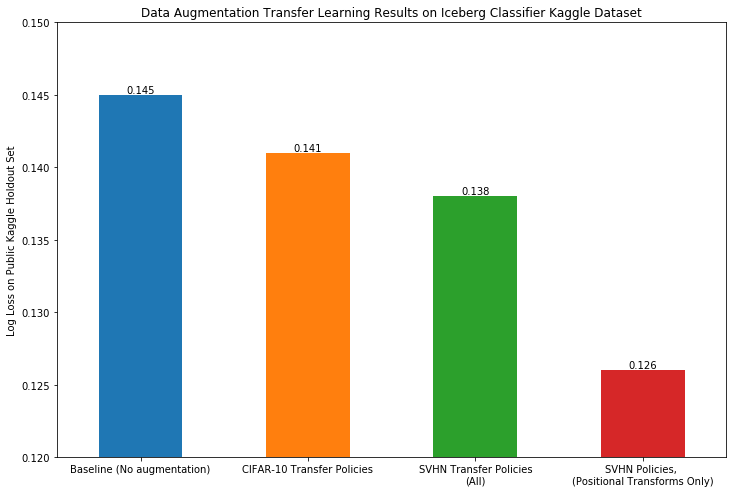
\includegraphics[width=\columnwidth]{iceberg_results.png}
\caption{Results When Transfering CIFAR-10 and SVHN Policies to Training on Iceberg Dataset}
\end{figure}

First we observe on visualizing the Iceberg data, the images are low color variation because they are fairly artificial "images" that were generated from radar readings. Given this observation, the relatively small improvements from transferring CIFAR-10 policies makes sense because those policies include many color-related augmentations such as Color, Brightness, AutoContrast, etc, as shown in Table 8 of the AugtoAugment paper [1].  

On the other hand, the improvements from using SVHN augmentations are almost twice as big, which makes sense because the SVHN augmentations contain relatively more positional transformations like ShearX, ShearY, Invert, Rotate, etc, as shown in Table 9 of the AutoAugment paper [1].  



\subsection{QuickDraw Dataset}

\begin{figure}[bhp]
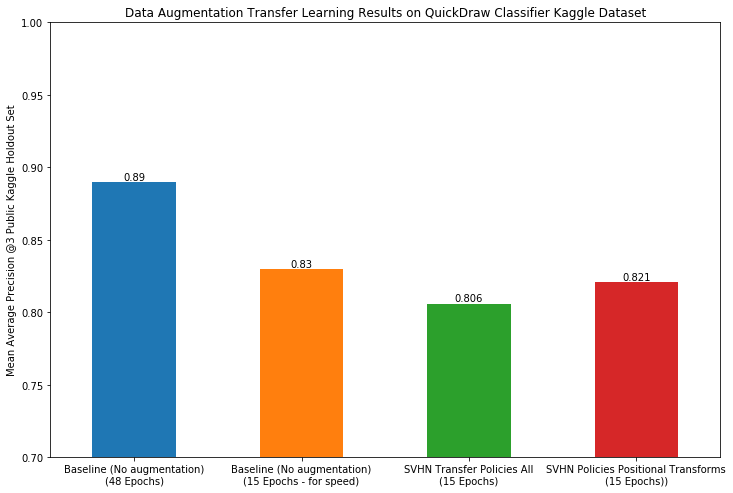
\includegraphics[width=\columnwidth]{quickdraw_results.png}
\caption{Results When Transfering Full and Partial SVHN Policies to Training on Iceberg Dataset}
\end{figure}

\section{Results - Simplified AutoAugment}


In our original proposal, we had planned to apply the AutoAugment [1] using the same Reinforcement Learning approach for finding the best policies that was suggested in the paper.  That proved to be difficult due to insufficient details in the paper, such as the number of epochs used in the Controller.  It would also require extensive computational resources to reproduce the exact results in the paper.

An alternative strategy we explored for automatic data augmentation was a random search over the set of all possible policies. We call this the "Simplified AutoAugment".  This strategy was inspired by random grid search for hyperparameter tuning, and it is much simpler than LSTM Controller. The constructed search space consists of the 16 policies, 10 and 11 discrete values for probability and magnitude respectively. On each epoch, a random policy is generated by uniformly sampling from each of these three random variables. A neural network is then trained on the CIFAR-10 dataset (reduced to 4000 random samples) using the chosen policy for auto-augmentation. The validation accuracy of the network is cached along with the chosen policy. The child network consists of 2 convolutional layers, a max pooling layer and a dropout layer, followed by a single dense layer and another dropout layer. The policy that produced the best accuracy is recovered after all epochs are complete.

The "Random Search Controller" was run for 250 epochs and kept track of the best policies it found for CIFAR-10. The policy that produced the best results was as follows:

\begin{itemize}
  \item Sub-Policy 0 = (Brightness, 0.1, 1.9), (ShearX, 0.0, -0.3)
  \item Sub-Policy 1 = (Invert, 0.7, 0.111), (Contrast, 0.5, 1.5)
  \item Sub-Policy 2 = (Invert, 0.3, 0.667), (Color, 0.5, 1.7)]
  \item Sub-Policy 4 = (Rotate, 1.0, 0.778), (ShearY, 0.3, -0.45)
  \item Sub-Policy 5 = (Brightness, 0.1, 1.5), (Invert, 0.9, 0.889)
 
\end{itemize}

The next steps for the final paper is to apply these top policies to the CIFAR-10 dataset and compare the results to the original AutoAugment.



\section{Results and Analysis}

\begin{figure}[bhp]
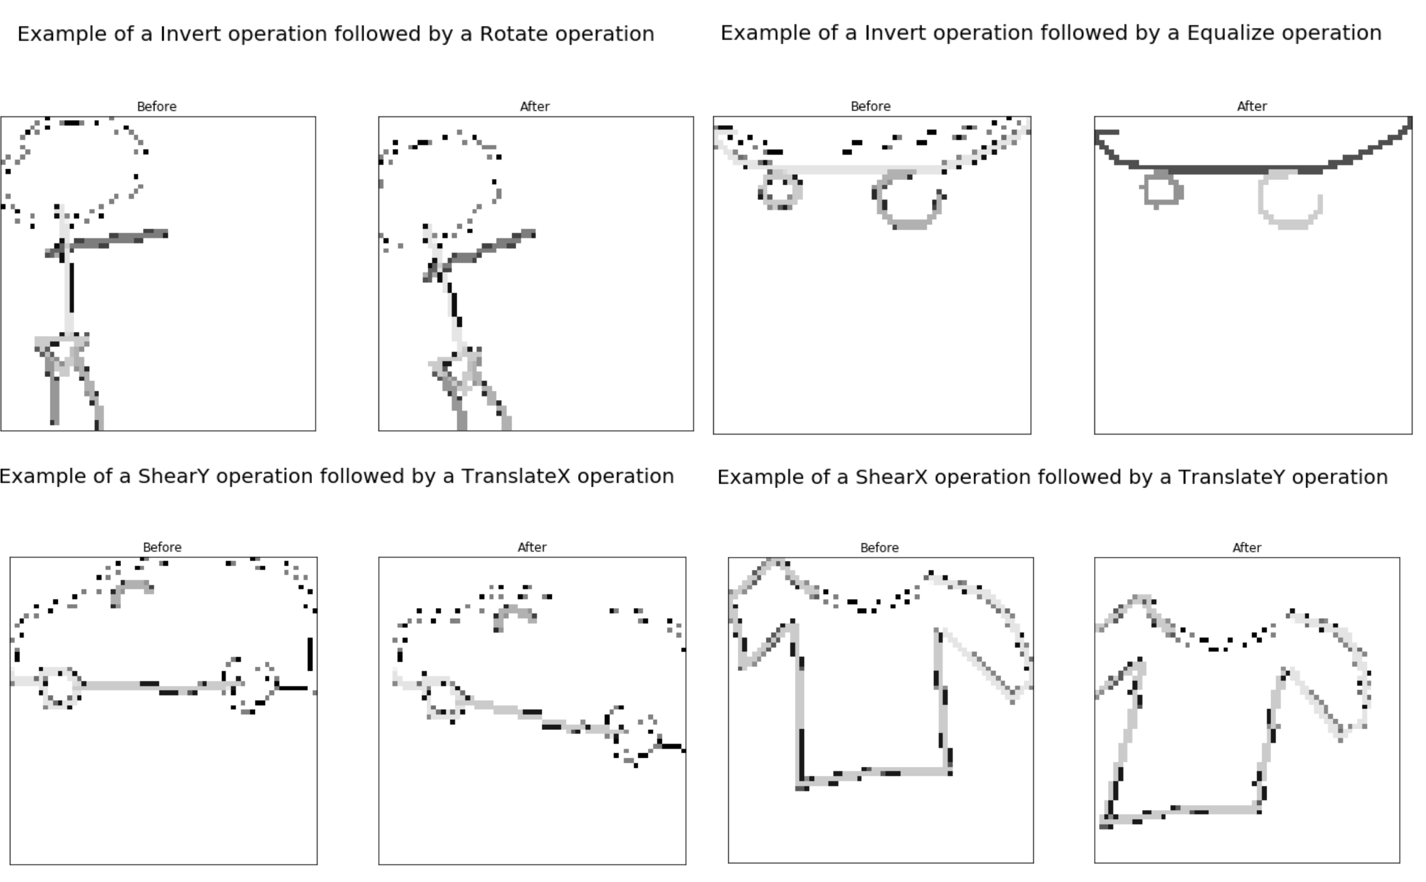
\includegraphics[width=\columnwidth]{quickdraw_compiled_transform_exmples.png}
\caption{Examples of Quickdraw Transformations}
\end{figure}


\section{Bitbucket Repository for This Paper}

The code for our project can be found at \url{https://github.com/rounakmehta/autoaugment_performance}. The repo contains scripts with implementations of the transfer learning and random search for policies. We have also cloned the original repository that the authors shared with the paper [1] in order to compare results. Because of the large size of the datasets, those were not included in the repo and need to be downloaded after cloning it. Instructions on the data download and details on how the repository structure can be found in the Readme.  

%-------------------------------------------------------------------------
\section{References}

[1]  E. D. Cubuk, B. Zoph, D. Mane, V. Vasudevan, and Q. V. Le. Autoaugment:   Learning  augmentation  policies  from  data, 2018. \newline
[2] B. Zoph, V. Vasudevan, J. Shlens, Q. V. Le. Learning Transferable Architectures for Scalable Image Recognition, 2017. \newline
[3] Ricardo Cruz, AutoAugment implementation, GitHub repository, https://github.com/rpmcruz/autoaugment, 2018 \newline

{\small
\bibliographystyle{ieee}
\bibliography{egbib}
}

\end{document}




